\documentclass{tudelftposter}
\usepackage{graphicx}
\usepackage{subfigure}
\title{TI2716-B License plate recognition, Poster 1}

\addauthornote{tu}{Group 8, Delft University of Technology}

\addauthor[tu]{Yinghao Dai}
\addauthor[tu]{Yanna van der Vlugt}

\addfootimage(c:right column.center)[Delft Institute of Applied Mathematics]{tudelft}


\begin{document}

\section{Introduction}


\section{License plate detection}
\begin{figure}[h]
	\centering
	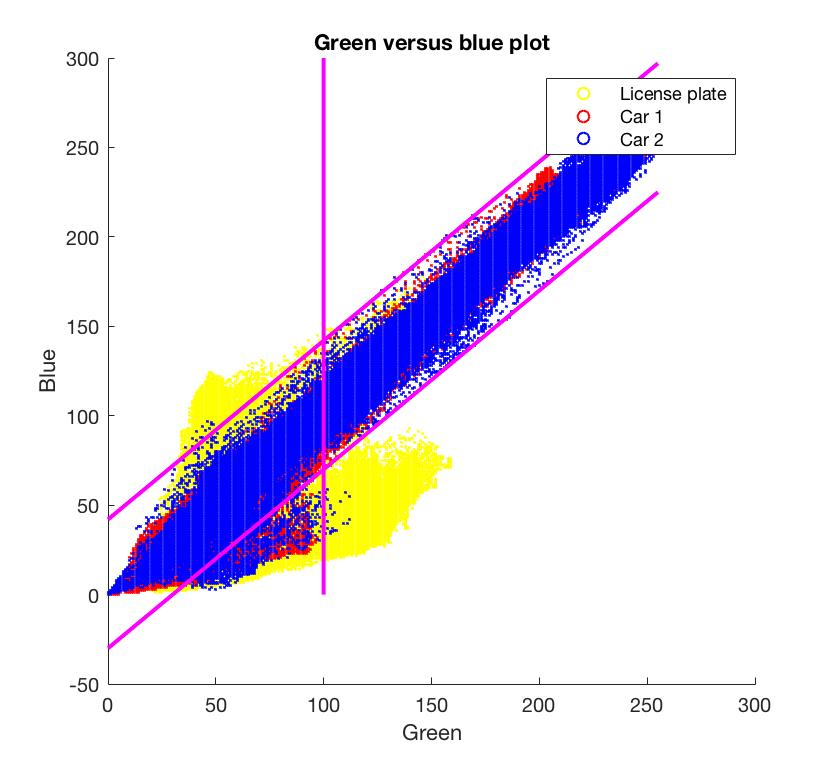
\includegraphics[width=1000pt]{greenblueplot.jpg}
	\caption{Scatterplot of different objects ($G$ value against $B$ value).}
	\label{greenblue}
\end{figure}

\section{Standardization}
\begin{figure}[h]
	\centering
	\subfigure[Original image]{
\includegraphics[width=500pt]{cropped.jpg}}
	\subfigure[After rotation]{
\includegraphics[width=500pt]{rotatedwrong.jpg}}
	\subfigure[After interpolation]{
\includegraphics[width=500pt]{rotated.jpg}}
	\subfigure[After labeling]{
\includegraphics[width=500pt]{labeledletters.jpg}}
	\caption{Process of standardizing a license plate.}
	\label{cropped}
\end{figure}

\section{GUI}


\section{Focus for next week}

\end{document}
%\experimentalblockright{%
%  SPAM:
%  Nulla malesuada porttitor diam. Donec felis erat, congue non, volutpat at,
%  tincidunt tristique, libero.}